\chapter{Grundlagen}
\section{Historie}
Seit dem Beginn des Industriezeitalters um 1800, welches mit der Mechanisierung (Industrie 1.0) startete, befindet sich die Industrie in einem stetigen Wandel. Sie entwickelte sich um 1900 durch die Massenproduktion zur Industrie 2.0 und in den 1970er Jahren durch die Automatisierung zur Industrie 3.0. Die Einteilung der Industriezeitalter ist durch tiefgreifende Veränderungen im technologischen Fortschritt möglich, welche auch als industrielle Revolution bezeichnet werden. Aktuell befinden wir uns in der Phase der 4. industriellen Revolution.

Die 1. industrielle Revolution fand mit der Erfindung der Dampfmaschine statt. Sie ermöglichte es Eisenbahnen und Dampfschiffe sowie verschiedene Maschinen im Kohleabbau oder in Textilfabriken anzutreiben und trug massiv zur Industrialisierung und der Entstehung der Industrie 1.0 bei. Nach und nach wurden immer mehr Produktionsanlagen errichtet und somit Arbeitsplätze in Infrastruktur, Textilfabriken, Häuserbau, Kohleabbau und anderen Bereichen geschaffen.

Die Erforschung der Elektrizität im 19. Jahrhundert war der Auslöser der 2. industriellen Revolution. Nachdem ab 1830 die Gesetze der Elektrotechnik bekannt waren, fand die Elektrizität eine breite Anwendung in der Industrie und im Alltag. Im Jahr 1913 führte Henry Ford das Fließband in der Automobilbranche ein. Im Zuge dessen musste jeder Arbeiter nur noch einen Arbeitsschritt erledigen, welches einerseits die Produktion wesentlich beschleunigte und eine Massenproduktion ermöglichte und andererseits eine hohe Spezialisierung der einzelnen Arbeitskräfte für ihre bestimmte Aufgabe erforderte. Außerdem wurde es durch die Luftfahrt möglich Produkte wie Autos, Kleidung und Lebensmittel über Kontinente hinweg immer schneller zu transportieren und zu handeln.

Die 3. industrielle Revolution fand in den 1970er Jahren statt. Sie ist durch eine sukzessive (Teil-) Automatisierung der Prozesse und durch den Einzug der IT in die Industrie- und Verbraucherwelt geprägt. In den 1940er Jahren wurden die ersten Rechenmaschinen und programmierbare Steuerungen in Unternehmen eingesetzt. In den 1970er Jahren zog der Computer auch in den Privatbereich ein, wurde zunehmend beliebter und schaffte einen neuen Industriezweig. Der Fertigungsprozess in Fabriken wurde mehr und mehr von Maschinen übernommen. Durch den zunehmenden Einsatz von IT in Unternehmen entstand immer mehr Kommunikation zwischen Menschen und Maschinen. Diese Kommunikation und die anfallenden Daten wurden jedoch nur unternehmensintern verarbeitet. Es gab nur wenige Schnittstellen nach außen.

Das Ende des 20. Jahrhunderts gilt als der Beginn der 4. industriellen Revolution. Das Kennzeichen dieser Phase ist die zunehmende Digitalisierung und der Einzug der Internet-Technologien in die Industrie. Mit ihr geht die technische Vernetzung physischer Gegenstände, dem \ac{IoT}, einher. Mehr und mehr Geräte oder Gegenstände besitzen die Möglichkeit aktiv über eine Netzwerkschnittstelle oder passiv mit Hilfe eines Bar- oder QR-Codes mit der digitalen Welt zu kommunizieren und somit eine fortschreitende Automatisierung und Individualisierung zu ermöglichen. Diese Entwicklung macht es möglich immer schneller Informationen auszutauschen, größere Datenmengen zu analysieren und diese zu verarbeiten. In der Industrie entstehen dadurch u. a. die folgenden Chancen:

\begin{itemize}
  \item Die Kommunikationsinfrastruktur wird in Zukunft in Produktionssystemen so preiswert sein, dass sie sinnvoll für Konfiguration, Service, Diagnose, Bedienung und Wartung genutzt werden kann.
  \item Die Produktionssysteme werden mehr und mehr mit einem Netz verbunden, erhalten dort eine digitale Identität, werden somit such- und analysierbar und besitzen die Möglichkeit Daten über sich selbst zu veröffentlichen. 
  \item Maschinen und Anlagen speichern ihre Zustände in ihrer digitalen Identität im Netz. Diese Zustände sind aktuell, aktualisierbar und zunehmend vollständig. Sind im Netzwerk viele solcher Identitäten vorhanden, können die Daten effizient abgerufen und ausgetauscht werden.
  \item Softwaredienste werden über das Netz verknüpft und können somit automatisiert individuelle Aufgaben durch die direkte Kommunikation der Systeme erledigen. Eine solche individuelle Wertschöpfung war bisher nur unwirtschaftlich oder gar nicht möglich.
\end{itemize}

Im Gegensatz zur Industrie 3.0 sollen Maschinen autonom, auch über Unternehmensgrenzen hinweg, miteinander kommunizieren können um gesamte Geschäftsprozesse zu übernehmen. Dies setzt eine Öffnung der Unternehmen nach außen voraus und wird in \autoref{Grundlagen:Industrie4.0-Kommunikation} dargestellt.

\begin{figure}[h]
  \centering
  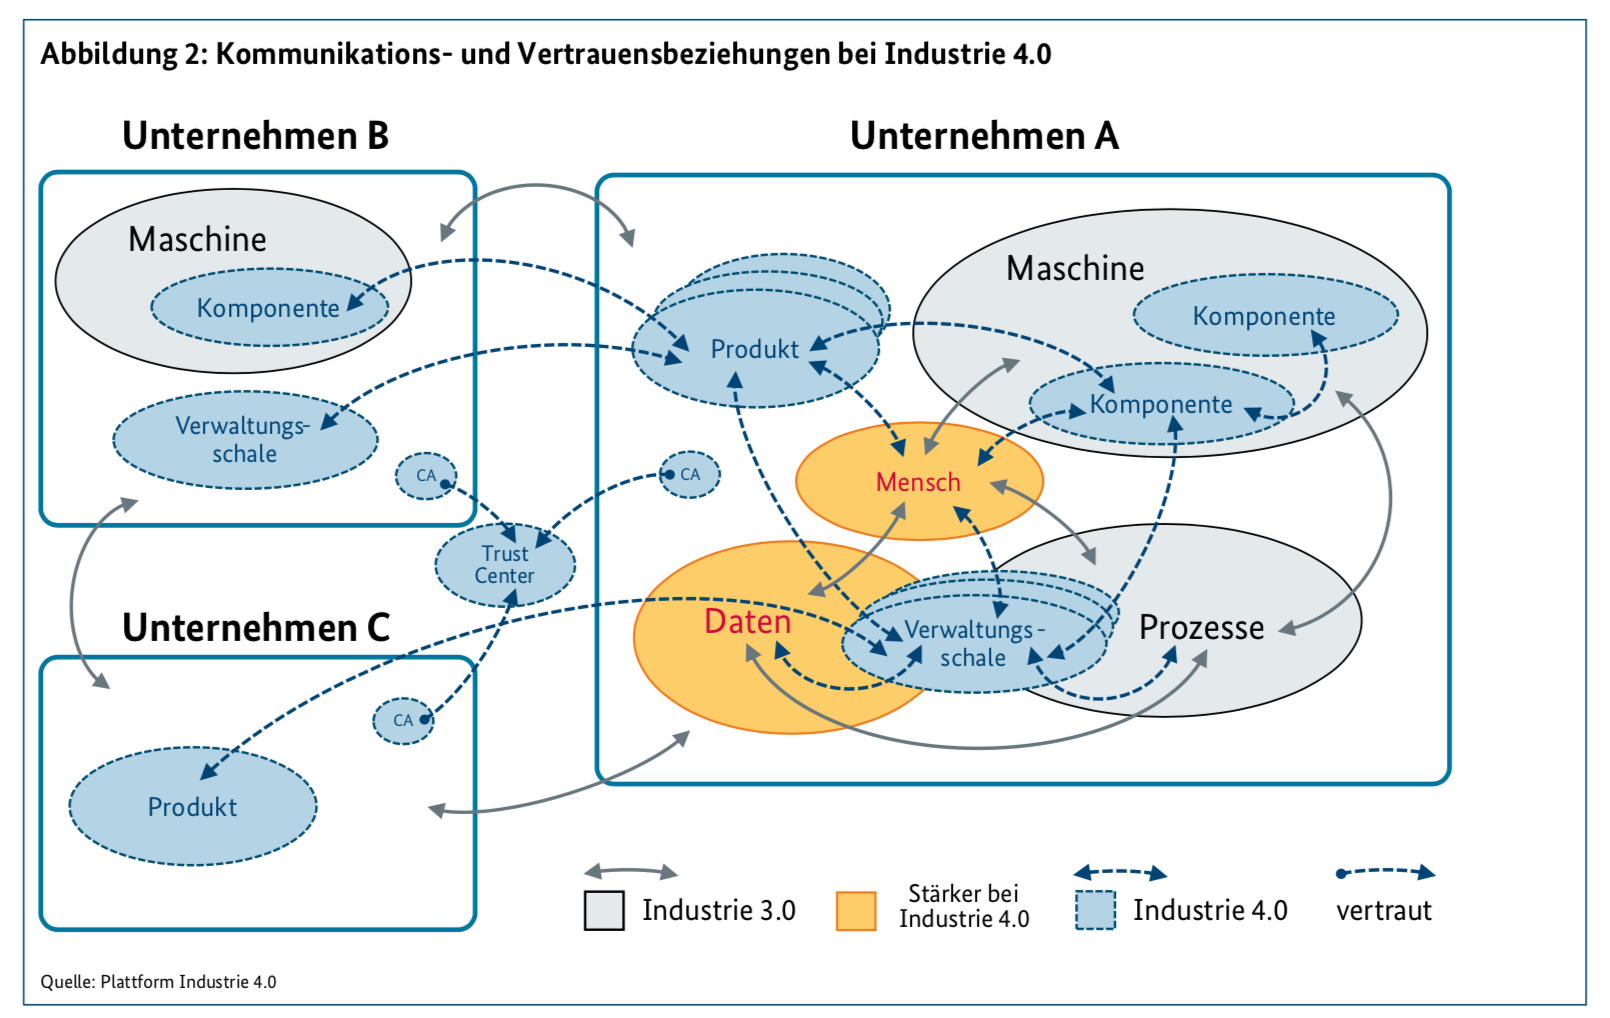
\includegraphics[width=15cm]{kommunikationsbeziehungen-i40}
  \caption{Kommunikationsbeziehungen in einer Industrie 4.0 Umgebung}
  \label{Grundlagen:Industrie4.0-Kommunikation}
\end{figure}

\clearpage

\section{Automatisierungspyramide}
\label{Grundlagen:Automatisierungspyramide}
Die Automatisierungspyramide (\autoref{Grundlagen:Automatisierungspyramide-img}) stellt die beteiligten Systeme und Softwarekomponenten eines automatisierten Prozesses dar. In der Industrie 4.0 wird eine automatisierte und direkte Kommunikation zwischen allen Ebenen der Automatisierungspyramide angestrebt. Die beteiligten Systeme beginnen, ausgehend vom Kundenauftrag und der betriebswirtschaftlichen Planung der Produktion auf der Unternehmensebene beim \ac{ERP} System. Die Ergebnisse der Planung werden an das \ac{MES} übergeben, welches die verschiedenen Fertigungs- oder Logistikaufträge generiert. Die Aufträge werden anschließend auf der Prozessleit- (\ac{SCADA}), Steuerungs- (\ac{SPS}) und Feldebene (Ein-/Ausgangssignale) mit Hilfe von Steuerungen und Sensoren bearbeitet. Während die oberen Schichten der Pyramide (\ac{ERP} und \ac{MES}) durch Standardkomponenten bzw. -software der IT realisiert werden, zählen die unteren Schichten (Prozessleit- bis Feldebene) zur Automatisierung, welche die Steuerung und Kontrolle der technischen Anlagen übernimmt. Sie sind durch spezielle Hard- und Softwarelösungen umgesetzt. Die Integration von Sicherheitsmaßnahmen bei der Kommunikation dieser Systeme stellt oft eine große Herausforderung dar, da besondere Anforderungen vorliegen oder wenig Ressourcen zur Verfügung stehen.

\begin{figure}[h]
  \centering
  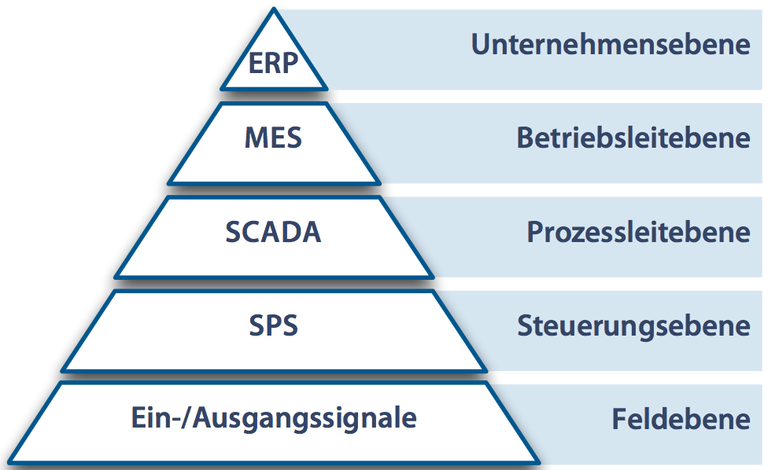
\includegraphics[width=10cm]{automatisierungspyramide}
  \caption{Automatisierungspyramide - TODO ref. Langmann,2004}
  \label{Grundlagen:Automatisierungspyramide-img}
\end{figure}

\clearpage

\section{Industrie 4.0}
Der Begriff Industrie 4.0 wurde erstmals auf der Hannover Messe 2011 verwendet (\cite{drath2014}) und soll das Ergebnis der 4. industriellen Revolution darstellen. Der Grundgedanke hinter Industrie 4.0 ist die flächendeckende Vernetzung von Informations- und Kommunikationstechnik zu einem Internet der Dinge, Dienste und Daten (\cite{spath2013}). Diese Vernetzung soll einen ständigen Informationsaustausch zwischen den Komponenten ermöglichen. Jede Komponente des \ac{IoT} soll als \ac{CPS} arbeiten. Ein \ac{CPS} besitzt neben seiner realen Identität eine digitale Identität, über welche es ständig mit anderen \ac{IoT}-Geräten kommunizieren kann. Kunden- und Maschinendaten werden miteinander vernetzt (\cite{rami2016}). Dieser Prozess beschreibt auch einen Wandel in der Strukturierung und Organisation der Produktion in Unternehmen. Durch die fortschreitende Automatisierung wird die Umsetzung einer immer höheren Individualisierung bei geringerer produzierter Stückzahl rentabel. \autoref{Grundlagen:Das Internet der Dinge} zeigt die Vernetzung der verschiedenen Industriesektoren und Komponenten über das \ac{IoT}.

\begin{figure}[h]
  \centering
  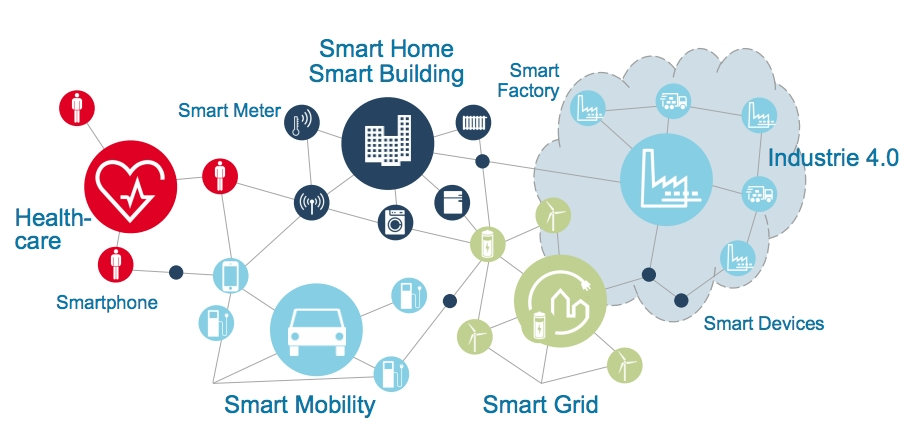
\includegraphics[width=15cm]{internet-der-dinge}
  \caption{Das Internet der Dinge}
  \label{Grundlagen:Das Internet der Dinge}
\end{figure}

\clearpage

\subsection{Internet of Things/Industrial Internet of Things}
\label{Grundlagen:IoT/IIoT}
Die fortschreitende Vernetzung der Komponenten spiegelt sich im \ac{IoT} bzw. \ac{IIoT} wieder. Das \ac{IoT} beschreibt im Gegensatz zum \ac{IIoT} ein verbraucherorientiertes Konzept für die Nutzung von digitalisierten und vernetzten Systemen. Hierbei werden die physischen Systeme virtuell abgebildet. Dies wird genutzt, um die Effektivität der Systeme zu verbessern und intelligente Services zu nutzen.

Das \ac{IoT} ist ein wesentlicher Bestandteil der Industrie 4.0, welche Netzwerke aus Systemen, Daten und Dienstleistungen herstellt, in denen diese Komponenten miteinander kommunizieren. Im Verbraucherbereich und für die Kommunikation zwischen Mensch und Maschine findet das Protokoll \ac{HTTP} und dessen \ac{REST} Programmierparadigma breite Anwendung. 

Das \ac{IIoT} beschreibt den Gebrauch von \ac{IoT}-Technologien im industriellen Raum. Diese Systeme können besondere Anforderung an die Kommunikation im Netzwerk wie Skalierbarkeit, Ressourcenverbauch, Echtzeitkommunikation oder Sicherheit stellen. Des Weiteren findet in Industrie 4.0 Umgebungen \ac{M2M} Kommunikation statt. Um diesen Problemen entgegenzuwirken, wurden neue Protokolle zur Übermittlung von Daten im Netzwerk entwickelt. Hierbei erfahren vor allem die Protokolle \ac{MQTT} und \ac{CoAP} ein hohes Maß an Beachtung. Diese Protokolle wurden für eine ressourcenschonende Kommunikation zwischen Maschinen entwickelt.

\subsection{Referenzarchitekturen}
Um eine flächendeckende Vernetzung der digitalen Komponenten zu ermöglichen, muss eine einheitliche Kommunikation geschaffen werden. Diese beschränkt sich nicht nur auf die Form der Nachrichten im Netzwerk und deren Gewährleistung der Sicherheit, sondern beinhaltet auch die Struktur und Bereitstellung von Informationen im Netzwerk. In der Folge wurden verschiedene Referenzarchitekturmodelle entwickelt, um Standards für die Kommunikation und Interaktion von Netzwerkkomponenten innerhalb einer Industrie 4.0 Umgebung zu definieren.

\subsubsection{\ac{RAMI4.0}}
\label{Grundlagen:RAMI4.0}
Das \ac{RAMI4.0} wird in der DIN SPEC 91345 beschrieben und dient als Konzept zur strukturierten Umsetzung der grundlegenden Idee hinter dem Begriff Industrie 4.0. Die Aufgabe des Architekturmodells ist es, die Ziele einer Industrie 4.0 Umgebung, die vollständige Vernetzung der physischer Wertgegenstände, umzusetzen. Diese Gegenstände werden im Rahmen der \ac{RAMI4.0} als \textit{Assets} bezeichnet. Jedes \textit{Asset} besitzt seine eigene Verwaltungsschalte, welche als Schnittstelle zum Austausch von Informationen dient. Die Verwaltungsschale soll eine standardisierte Kommunikation und einfache Inbetriebnahme neuer Komponenten ermöglichen (\cite{rami2016}). Mit Hilfe der \ac{RAMI4.0} soll es möglich  den Status eines \textit{Assets} zu jedem Zeitpunkt im Lebenszyklus nachweisen zu können. Die \ac{RAMI4.0} ist in \autoref{Grundlagen:RAMI4.0-img} dargestellt und wird durch ein Modell aus sechs Schichten und drei Achsen dargestellt. (\cite{RAMISpec})

Auf der Architekturachse werden sechs Schichten beschrieben. Auf der untersten Schicht wird der Gegenstand der physischen Welt dargestellt. Alle zu ihm relevanten Information werden in den darüberliegenden Schichten gespeichert. Darüber stellt die \textit{Integration} Schicht das Bindeglied zwischen der physischen und digitalen Welt bereit, indem sie die Eigenschaften des \textit{Assets} für Computersysteme erreichbar macht (\cite{BMWiNeCon2016}). Die \textit{Communication} Schicht beschreibt den Zugriff auf die Ressourcen und Funktionen der Komponente und stellt die Dienste einer \ac{SOA} bereit. Auf der \textit{Information} Schicht wird die Funktionalität des \textit{Assets} gespeichert und die Datenintegrität gewährleistet. Die \textit{Functional} Schicht beschreibt die Form, wie und mit welchen Parametern ein Funktionsaufruf stattfinden kann. In der \textit{Business} Schicht werden die geschäftsrelevanten Daten gehalten. (\cite{RAMISpec})

Die Hierarchieachse zeigt die Anlagen, Maschinen sowie das Endprodukt, welche miteinander Vernetzt sind. Die in \autoref{Grundlagen:Automatisierungspyramide} beschriebene Automatisierungspyramide findet sich in der Hierarchieebene der \ac{RAMI4.0} wieder. Sie wurde dort auf der niedrigsten Ebene um das Produkt (\textit{Product}) sowie auf der höchsten Ebene um die Stufe \textit{Connected World} erweitert. Die \textit{Connected World} beschreibt den Zusammenhang zwischen einem Asset oder einer Assetkombination und einem anderen Asset oder einer Assetkombination, also einem Fabrikverbund. (\cite{RAMISpec})

Der Produktlebenszyklus wird im Gegensatz zur Industrie 3.0 in das Netzwerk mit eingebunden. Der gesamte Prozess der Produktion, Wartung bis hin zur Verschrottung wird digital erfasst. Somit könnten ständig Informationen über vorhandene \textit{Assets} gesammelt und zur Optimierung des Werschöpfungsprozesses analysiert werden. (\cite{RAMISpec})

\begin{figure}[h]
  \centering
  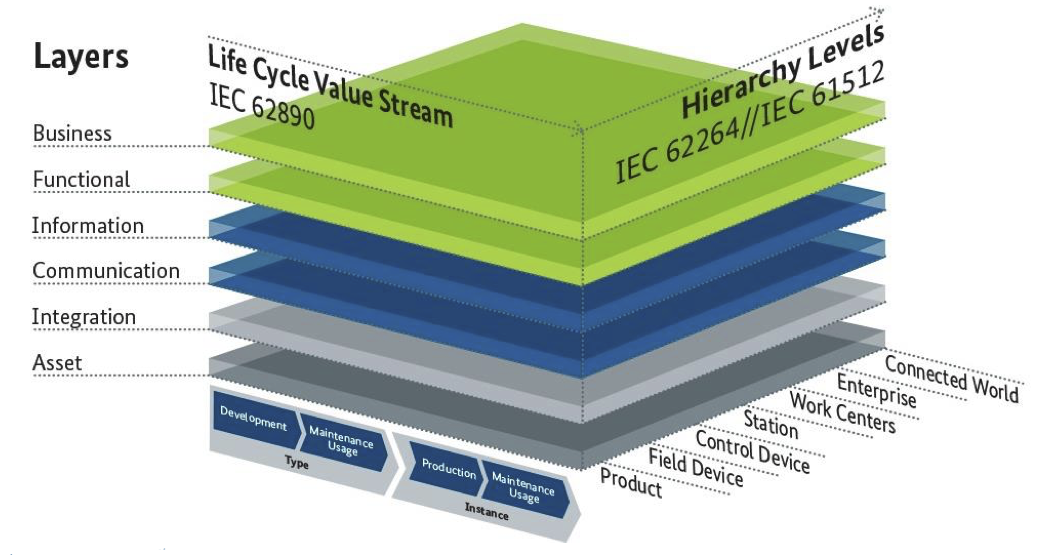
\includegraphics[width=15cm]{rami40}
  \caption{RAMI 4.0}
  \label{Grundlagen:RAMI4.0-img}
\end{figure}

\clearpage

\subsubsection{IIRA}
\label{Grundlagen:IIRA}
Das \ac{IIC} veröffentlichte im Jahr 2015 die \ac{IIRA}. Die \ac{IIRA} beschreibt eine standardbasierte, offene Referenzarchitektur für \ac{IIoT}, welches auf dem \ac{IIAF} basiert. Das \ac{IIAF} unterstützt die Unternehmen bei der Entwicklung, Dokumentation, Kommunikation und Bereitstellung von Systemen im \ac{IIoT} Bereich (\cite{iira2017}). Die Beschreibung der Architektur findet mit einem hohen Maß an Abstraktion statt, um das breite Feld der verschiedenen Industrielösungen abdecken zu können und standardisierte Vorgehensweisen zu ermöglichen. Das \ac{IIAF} folgt der Vorgehensweise des ISO/IEC/IEEE Standard 42010:2011\footnote{ISO/IEC/IEEE Standard 42010:2011 - Systems and Software Engineering–Architecture Description}. Hieraus werden die grundlegenden Architekturbeschreibungskonstrukte \textit{Concern}, \textit{Stakeholder} und \textit{Viewpoint} übernommen. Die \textit{Viewpoints} sind die grundlegenden Ebenden beim Aufbau der \ac{IIRA}. Dabei werden vier \textit{Viewpoints} für die Beschreibung festgelegt. (\cite{heidrich2016})

Der \textit{Business Viewpoint} beinhaltet die betriebswirtschaftlichen \textit{Concerns} bei der Umsetzung eines \ac{IIS} sowie die entstehenden Rahmenbedingungen. Es werden die Systemeigenschafen definiert, welche an die Geschäftsziele gekoppelt sind. Die \textit{Stakeholder} dieses \textit{Viewpoints} bestehen aus Führungskräften, Produktmangern und Systemingenieuren.

Im \textit{Usage Viewpoint} werden die \textit{Concerns} bei der Nutzung eines \ac{IIS} beschrieben. Dies beinhaltet die Beschreibung der Bedienabläufe.

Der \textit{Functional Viewpoint} beschreibt die funktionalen Komponenten des \ac{IIS}. Es werden Zusammenhänge, Struktur, Schnittstellen und Interaktionen mit Systemen im Netzwerk sowie der Außenwelt beschrieben.

Der \textit{Implementation Viewpoint} beinhaltet die Technologien zur Umsetzung des \ac{IIS}. Es werden die funktionalen Komponenten, deren Vernetzung, Kommunikationsschnittstellen sowie deren Produktlebenszyklen dargestellt. Diese \textit{Concerns} sind wichtige Ansatzpunkte für Komponentendesigner, Systementwickler und Integratoren. 

\begin{figure}[h]
  \centering
  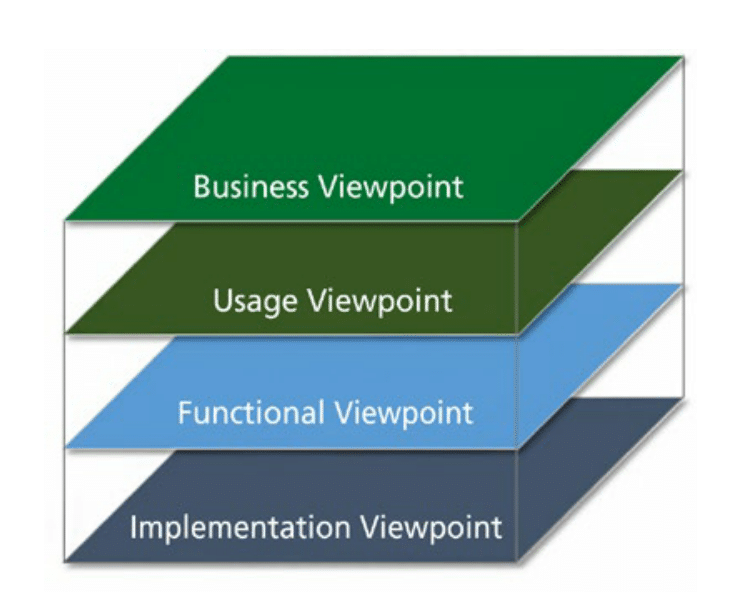
\includegraphics[width=10cm]{iira}
  \caption{Die Grundebenen der IIRA} 
  \label{Grundlagen:IIAF/IIRA - Übersicht}
\end{figure}

\clearpage

Die Anforderungen des Referenzarchitekturmodells beinhalten niedrige Latenzen und Schwankungen, einen hohen Durchsatz, Skalierbarkeit, Ausfallsicherheit, Datensicherheit und \ac{QoS}. Die \ac{IIRA} stellt einen softwaretechnischen Ansatz der Darstellung einer Referenzarchitektur bereit.

\subsection{Kommunikationsstrukturen}
\label{Grundlagen:Kommunikationsstrukturen}
TODO

\subsubsection{End2End}
\label{Grundlagen:End2End}
Die Komponenten der Industrie 4.0 Umgebung kommunizieren über einen direkten Kanal miteinander. Dies setzt voraus, dass sich beide Teilnehmer in einem Netzwerk befinden, welches die benötigten Dienste wie z. B. \ac{IP} und \ac{DNS} zur Kommunikation bereitstellt. Des weiteren müssen beide Systeme diese Dienste und Protokolle unterstützen.

\subsubsection{Gateways}
Um existierende Systeme, welche selbst nicht Industrie 4.0 konform kommunizieren oder zu wenig Rechenleistung besitzen, in die Industrie 4.0 Welt zu integrieren, werden Industrie 4.0 Gateways genutzt. Dabei ist jedoch zu beachten, dass die Systeme hinter den Gateways nicht als Industrie 4.0 Komponenten entwickelt wurden und somit auch keine oder nur wenige dieser Eigenschaften besitzen. Des Weiteren ist es möglich, dass die Kommunikation aus Leistungsgründen oder besonderer Anforderungen über optimierte, proprietäre Protokolle stattfindet. Die Gateways müssen auf die Systeme und deren Protokolle individuell konfiguriert werden, um die Funktionalitäten im Industrie 4.0 Netz bereitstellen zu können, und die Kommunikation zu schützen.

\subsubsection{Publish-Subscribe}
\label{Grundlagen:Publish-Subscribe}
Das Publish-Subscribe Modell bietet die Möglichkeit Informationen an mehrere Teilnehmer zu verteilen. Hierbei melden sich die Empfänger beim Verteiler an und wählen aus, über welche Nachrichtentypen sie informiert werden möchten. Diese Verteildienste nutzen zur besseren Skalierung und Reduzierung der Netzlast häufig Datagramme wie \ac{UDP}. Durch die Nutzung von Datagrammen geht jedoch die Fehlertoleranz verloren. Somit muss entweder dafür gesorgt werden, dass eine sehr zuverlässige Netzwerkinfrastruktur vorhanden ist und hohe Bandbreitenreserven geschaffen werden, um die Dienstgüte (\ac{QoS}) sicherzustellen oder dieses Modell nur für fehlertolerante Kommunikation wie z. B. Audio- und Video-Anwendungen oder Businessprozesse zu nutzen. 

\subsubsection{Kommunikation mit Netzwerk als Partner}
Zeitkritische Automatisierungsanwendungen verlangen besondere Netzwerkeigenschaften. Sie können auf Latenz oder Jitter angewiesen sein. Um diese Eigenschaften sicherzustellen, ist es sinnvoll in diese Netze eine Industrie 4.0 Schnittstelle zu integrieren. Somit ist es den Teilnehmern möglich, über die Verwaltungsschale sicherzustellen, dass das Netzwerk die erforderlichen Anforderungen bereitstellt. (\cite{sichKom2017})

\subsection{Protokolle}
Die Kommunikation in Industrie 4.0 Umgebungen findet nicht mehr über einzelne, vorgegebene Schnittstellen statt, sondern direkt von den Produktionssystemen, also den unteren Ebenen der Automatisierungspyramide. Um dies zu ermöglichen, ist es notwendig, eine einheitliche Kommunikation durch Normen und Standards herzustellen, um eine unternehmensübergreifende Kommunikation aller Komponenten zu ermöglichen. Durch die in der Industrie 4.0 benötigte \ac{M2M} Kommunikation wurde die Entwicklung neuer Protokolle zum effizienten Informationsaustausch vorangetrieben, welche es ermöglichen sollen, eine Standardisierung bereitzustellen und somit eine herstellerübergreifende und plattformunabhängige Kommunikation zu ermöglichen. Hierbei haben sich bzgl. der Referenzarchitekturen \ac{RAMI4.0} und \ac{IIRA} die Protokolle \ac{OPC UA} und \ac{DDS} etabliert.

\subsubsection{\ac{OPC UA}}
\ac{OPC UA} ist in der \ac{IEC} 62541 als offener Standard definiert und erstreckt sich über Communication- und Information Layer des \ac{RAMI4.0}. Es vereint Daten- und Informationsdienste und stellt einen sicheren, zuverlässigen und plattformübergreifenden Informationsaustausch zwischen unterschiedlichen Geräten und Systemen der Industrie bereit. Die \ac{OPC UA} ermöglicht die Kommunikation über die verschiedenen Schichten der Automatisierungspyramide von der Feldebene bis zur Unternehmensebene. 

\ac{OPC UA} wurde ursprünglich als Client-Server Architektur entwickelt. Um \ac{OPC UA} besser in Systemen der unteren Ebenen der Automatisierungspyramide, wie Kleinsteuerungen, Sensoren und Low-End-Embedded-Systeme, einsetzen zu können, werden meist geringe Latenzen in den Netzwerken und ein geringer Overhead aufgrund von Ressourcenmangel sowie die Kommunikation mit mehreren Partnern benötigt. Diese Anforderungen wurden von dem im Jahr 2018 veröffentlichten 14. Teil der \ac{OPC UA} Spezifikation \textit{Publish Subscribe} adressiert. Das \textit{Publish Subscribe} Modell wird mit Hilfe des Transportprotokolls \ac{UDP} umgesetzt und ermöglicht den Multi- und Broadcast sowie die Möglichkeit der häufigen Übertragung von kleinen Datenmengen um \textit{Logging} oder \textit{Monitoring} durchzuführen, ohne das Netzwerk durch einen 3-Wege-Handshake bei jedem Verbindungsaufbau zusätzlich zu belasten (\cite{opcpt1}).

\ac{OPC UA} stellt ein Informationsmodell mit Hilfe einer \ac{SOA} bereit, erfüllt die Anforderungen des \ac{RAMI4.0}, etabliert sich zunehmend im Maschinen- und Anlagenbau und bietet einen vielversprechenden Ansatz für einen standardisierten Informationsaustausch über Unternehmensgrenzen hinweg (\cite{OPCWegbereiter2014}). Aufgrund dessen stellt es auch ein attraktives Ziel für Industriespionage und die Sabotage von Industrienetzen bereit (\cite{opcpt2}). 

\ac{OPC UA} wird in 14 geschichteten Spezifikationen beschrieben, welche sich in die Bereiche \textit{Core}, \textit{Access Type} und \textit{Utility} unterteilen lassen. Dabei stellen die Spezifikationen 1-7 sowie 14 die Kernfunktionalitäten des Architekturmodells dar. Sie beschreiben die Struktur des OPC Addressraums und der Dienste, die darauf operieren. Die Spezifikationen 8-11 wenden diese Kernfunktionalitäten auf spezifische \ac{OPC COM} Spezifikationen, wie \ac{DA}, \ac{AE} und \ac{HDA} an. Die Teile 12 und 13 beinhalten Mechanismen zur Discovery von Systemen und beschreiben Möglichkeiten der Datenaggregation.

\begin{figure}[h]
  \centering
  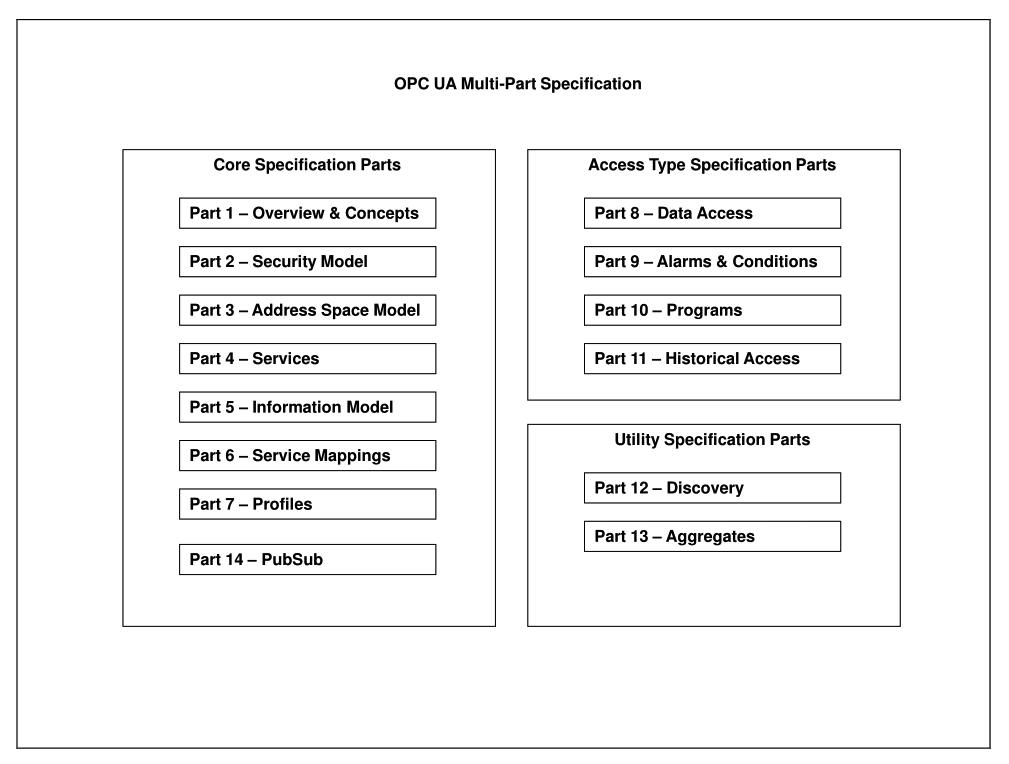
\includegraphics[width=15cm]{opcua-spezifikation}
  \caption{OPC UA Multi-Part Specification - \cite{opcpt1}} 
  \label{Kap2:OPC UA Multi-Part Specification}
\end{figure}

\clearpage

Das Lesen- und Schreiben von Daten und die Kommunikation in Industrie 4.0 Umgebungen findet nach \ac{RAMI4.0} durch die Verwaltungsschale der Komponenten statt. Diese wird im \ac{OPC UA} Stack durch den Adressraum beschrieben. Der Adressraum wird zur Speicherung von Knoten, deren Attribute und Referenzen zu anderen Knoten genutzt. Der Addressraum und das Informationsmodell von \ac{OPC UA} werden in den Spezifikationen 3 \cite{opcpt3} und 5 \cite{opcpt5} definiert.

\ac{OPC UA} ermöglicht die Kommunikation der Assets über ein Client-Server Pattern. Die Architektur setzt sich dabei aus einem \ac{OPC UA} Client und einem \ac{OPC UA} Server zusammen. Der \ac{OPC UA} Server stellt verschiedene Funktionen bereit, auf welche der \ac{OPC UA} Client mit Hilfe eines Request zugreifen kann. Des Weiteren ist es möglich durch einen Request des \ac{OPC UA} Clients ein Element des Servers beobachten zu lassen, um bei Änderungen vom Server benachrichtigt zu werden. Um die Kommunikation zwischen \ac{OPC UA} Servern zu gewährleisten, wird ein \ac{OPC UA} Client in einen \ac{OPC UA} Server integriert. In der Grafik \autoref{Kap2:OPC UA Client-Server Architektur} wird das Client-Server Pattern der \ac{OPC UA} Spezifikation schematisch dargestellt. Die linke Seite der Grafik beschreibt die Kommunikation zwischen einem Client und einem Server mit eingebettetem Client. In der rechten Seite der Grafik findet die Kommunikation zwischen dem eingebetteten Client und einem \ac{OPC UA} Server statt.

\begin{figure}[h]
  \centering
  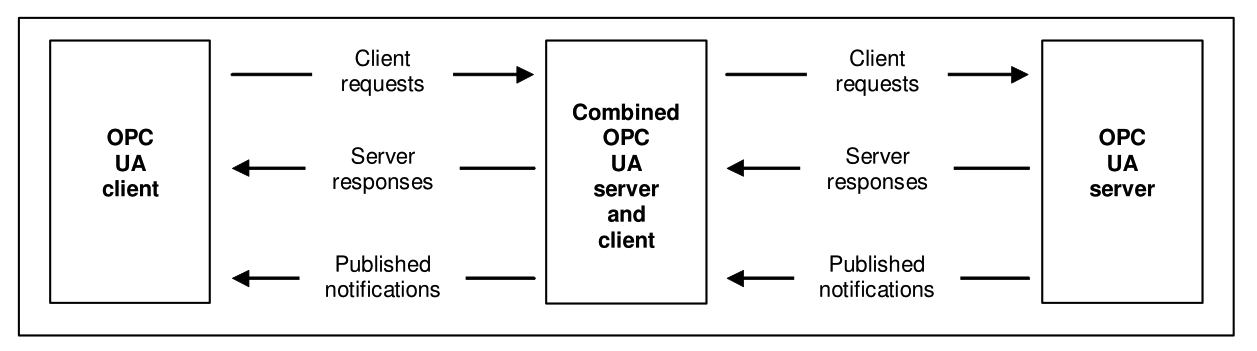
\includegraphics[width=15cm]{opcuaclient-server}
  \caption{OPC UA Client-Server Architektur - \cite{opcpt1}} 
  \label{Kap2:OPC UA Client-Server Architektur}
\end{figure}

\clearpage

Im Jahr 2018 wurde der Standard zusätzlich um eine Spezifikation für das Publish-Subscribe Modell erweitert (\cite{hoppe2018}). Das Publish-Subscribe Modell ermöglicht die Nutzung von \ac{OPC UA} in \ac{WAN} Umgebungen und die Verwendung von Protokollen wie \ac{MQTT} und \ac{AMQP}, während die Ende zu Ende Sicherheit und die standardisierte Datenmodellierung erhalten bleiben. Im Publish-Subscribe Modell wird das fehlertolerante Datagramm \ac{UDP} als Transportprotokoll verwendet, wodurch geringe Latenzen bei der Kommunikation ermöglicht werden.

\subsubsection{\ac{DDS}}
\ac{DDS} ist ein weiterer offener Standard der \ac{OMG} und stellt eine \ac{MOM} zur Kommunikation in hochdynamischen verteilten Systemen dar. Er wurde für niedrige Latenzzeiten, einen hohen Datendurchsatz und eine skalierbare, belastbase und sichere Datenverteilung entwickelt, um die Kommunikation in Steuerungs- und Kontrollaufgaben zu realisieren. Der beschriebene Standard deckt alle Anforderungen der \ac{IIRA} ab und hat sich bereits in industriellen Systemen etabliert. Gegenüber \ac{OPC UA} beschreibt \ac{DDS} eine dezentralisierte Architektur. Es bietet ein Konnektivitäts-Framework, welches ein Kommunikationsparadigma basierend auf einem Shared Data Model, einen Standard für die Definition domain-spezifischer Informationsmodelle, ein starkes Sicherheitsmodell, Discovery und reichhal­tige APIs beinhaltet. Die Kommunikation findet direkt vom Publisher zum Subscriber statt. Dabei werden Latenzzeiten reduziert und durch die Nutzung von Broad- und Multicast die Netzlast beim Bereitstellen von Informationen an viele Empfänger gering gehalten. Es ist möglich die \ac{MOM} \ac{DDS} in eine \ac{OPC UA} Architektur zu integrieren und mit dem Informationsmodell nutzen.

\subsection{Anforderungen an die Netzwerkkommunikation}
\label{Grundlagen:Anforderungen}
Aufgrund der unterschiedlichen Einsatzbereiche von Industrie 4.0 Systemen, unterscheiden sich auch dementsprechend deren Anforderungen. Um eine sichere Kommunikation in diesen Umgebungen bereitzustellen dienen die Grundprinzipien der sicheren Kommunikation. Die Referenzmodelle \ac{RAMI4.0} und \ac{IIRA} beschreiben ebenfalls drei Anforderungen an den Übertragungskanal: Sicherheit, Verfügbarkeit und \ac{QoS} (\cite{BMWiNeCon2016}).

TODO - grundprizipien der Sicheren Kommunikation kurz dann, auf anforderungen von RAMI und IIRA eingehen.!
TODO - in Bezug auf Industrie 4.0 ... oder Anforderungen an Industrie 4.0 Umgebungen basieren auf Grundprinzipien der sicheren Kommunikation
Die Grundprinzipien der sicheren Kommunikation beschreiben die Schutzziele im Bereich der Informationssicherheit. Diese verdeutlichen den Anspruch an die Sicherheit an ein zu implementierendes System oder ein Netzwerk. Sie stellen einen vereinbarten Umfang gegen Bedrohungen dar, welcher von den Kommunikationspartnern gewährleistet wird und nachgewiesen werden kann. Diese klassischen Schutzziele sind auch für Industrie 4.0 Umgebungen zutreffend. Die weitreichende Vernetzung der Systeme in der Industrie 4.0 erfordert jedoch weitere Schutzziele, um einen rechtskonformen Umgang oder besondere Anforderungen sicherzustellen.

TODO - Hierunter fallen die Bereiche Netzsicherheit und Datensicherheit, Sichere Identitäten und funktionale Sicherheit. Netzsicherheit und Datensicherheit werden in der AG3 der Plattform Industrie 4.0 adressiert. Die UAG Netzkommunikation arbeitet bzgl. dieser Punkte mit der AG3 zusammen. Zum Thema „Security und funktionale Sicherheit“ arbeitet die AG3 mit dem DKE-TBINK AK IT Security und Security by Design zusammen. Hinsichtlich funktionaler Sicherheit gibt es Anforderungen von Seiten IEC 61784-3. Diese müssen bei der Definition neuer Systeme berücksichtigt werden. - TODO

\begin{itemize}
  \item Vertraulichkeit/Zugriffsschutz
  \item (Daten)-Integrität/Änderungsschutz
  \item Authentizität/Fälschungsschutz
  \item Verfügbarkeit
\end{itemize}

\subsubsection{Sicherheit}
\begin{itemize}
    \item Netzsicherheit und Datensicherheit
    \item Sichere Identitäten
    \item funktionale Sicherheit
\end{itemize}

\subsubsection{Verfügbarkeit}
Die ständige Verfügbarkeit von Daten und Diensten spielt in der Industrie 4.0 eine bedeutende Rolle, um den Datenaustausch zwischen zwei Kommunikationspartnern im Netz jederzeit zu ermöglichen. Als Verfügbarkeit wird die Wahrscheinlichkeit bezeichnet, dass ein System innerhalb eines bestimmten Zeitraumes erreichbar ist. Ein System gilt als verfügbar, wenn es erreichbar ist und die für es vorgesehenen Aufgaben erledigen kann.

Die Verfügbarkeit eines Systems wird in Verfügbarkeitsklassen gegliedert. Diese beschreiben Verfügbarkeitswahrscheinlichkeiten von 99\% ( Verfügbarkeitsklasse 2 ) bis 99,9999\% ( Verfügbarkeitsklasse 6 ). Eine exakte Definition, wann ein System hochverfügbar ist, gibt es nicht - TODO ref. Im Allgemeinen wird ab Verfügbarkeitsklasse 3 ( 99,99\% ) von Hochverfügbarkeit gesprochen.

TODO - Verfügbarkeit gewährleisten durch...

\subsubsection{\ac{QoS}}
TODO - \ac{QoS}

\section{TCP/IP Referenzmodell}
\label{Grundlagen:TCP/IP Referenzmodell}
TODO - Das \ac{TCP}/\ac{IP} Referenzmodell stellt die Basis für moderne Kommunikationsnetze dar.
Unternehmensübergreifende Kommunikation in Industrie 4.0 Umgebungen findet im wesentlichen über IP-Netze statt. Diese basieren auf dem TCP/IP Referenzmodell, welches ein Schichtenmodell ist und die vier Schichten der Internetprotokollfamilie beschreibt. Sie setzen sich aus Application-, Transport-, Internet- und Link-Layer zusammen. Die Schichten des TCP/IP Referenzmodells überlagern sich mit den Schichten des ISO/OSI Referenzmodells. 

\subsubsection{Application Layer}
Die Anwendungsschicht ist für die Übertragung der Nutzdaten zwischen verschiedenen Anwendungen zuständig. Dabei kann es sich um entfernte Anwendungen handeln. Diese sollen sich für den Benutzer verhalten, als würden sie lokal ausgeführt werden.

TODO - Prozess- und Businesslogik

\subsubsection{Transport Layer}
Die Transportschicht sorgt für die Kommunikation zwischen Prozessen. Die Transportschicht nutzt Ports um verschiedene Dienste zu adressieren. Sie beeinflusst, ob es sich um eine zuverlässige Verbindung ( TCP ) oder nicht ( UDP ) handelt.

TODO - End2End Security

\subsubsection{Internet Layer}
Die Internetschicht wird genutzt, um Daten von einem Teilnehmer im Netzwerk zum anderen zu übertragen. Die Endpunkte im Netzwerk werden durch IP Adressen beschrieben.

\subsubsection{Link Layer}
Der Bitübertragungsschicht beschreibt die Topologie des Netzwerks. Sie stellt die physikalische Verbindung der Netzwerkteilnehmer zur Verfügung.

TODO - Bild Internetprotokollfamilie
TODO - Mit Bild nur kurz erklären und referenzieren, Überschriften entfernen.

\section{Security by Design}
\label{Grundlagen:Security by Design}
In der Vergangenheit wurden Sicherheitsmechanismen üblicherweise nachträglich und reaktiv in die Entwicklung von Komponenten mit einbezogen. Industrie 4.0 Umgebungen erfordern umfassende Maßnahmen, um die in \autoref{Grundlagen:Anforderungen} beschriebenen Schutzziele zu erfüllen und eine sichere Kommunikation zu gewährleisten. Dies gilt vor allem für Maschinenbau- und Fertigungsunternehmen, welche häufig proprietäre Individualsoftware zur Steuerung der Maschinen einsetzen (\cite{DTAG2016}). Aus der Notwendigkeit, Sicherheitsaspekte bereits in die Softwareentwicklung mit einzubeziehen und einen Schutz der Kommunikation zu gewährleisten, hat sich der Begriff \textit{Securiy by Design} entwickelt.

Die Methoden und Ziele der Angreifer stehen unter einem ständigen Wandel. Somit ist es nicht möglich, eine Sicherheitsimplementierung zu entwickeln und diese wiederholt einzusetzen. Vielmehr ist es notwendig, die Sicherheit durch \textit{Security by Design} so weit als möglich proaktiv herzustellen und gleichzeitig im Schadensfall flexibel zu reagieren, um das Schadensausmaß zu begrenzen. Es sind Maßnahmen zur Prävention, Detektion und Reaktion erforderlich (\cite{Umsetzung2015}). 

Das Konzept \textit{Security by Design} wird von \ac{RAMI4.0} und \ac{IIRA} sowie von den darin genutzten Protokollen \ac{OPC UA} und \ac{DDS} verfolgt. Die Absicherung der Kommunikation im Netzwerk gehört zu den Kernbestandteilen der Referenzarchitekturen (\cite{iirasec2017} und \cite{opcpt2}).

\section{Testsystem}
\label{Grundlagen:Testsystem}
TODO - kürzer

Die aus der Analyse hervorgehenden möglichen Schwachstellen und Bedrohungen im Bereich der Netzwerksicherheit in Industrie 4.0 Umgebungen und deren Auswirkungen sollen anhand eines vorhandenen, prototypischen Industrie 4.0 Testsystems (\cite{Weber2018}) veranschaulicht werden. Das vorhandene System setzt die drei Schichten der Software-Architektur (Verteilungs-, Baustein- und Laufzeitschicht) nach Starke / Hruschka um. Die Netzwerkkommunikation wird über das Protokoll \ac{OPC UA} realisiert, welches die Anforderungen der Industrie 4.0 und \ac{RAMI4.0} umsetzt.

TODO - Architektur
Das vorhandene System ist, aufgrund der vorgesehenen Einsatzgebiete Lehre, Integrations- und Sicherheitstests, als \ac{VM} umgesetzt worden. Dies ermöglicht es die Testinfrastruktur vom restlichen Netz zu kapseln. Das Betriebssystem der \ac{VM} stellt eine Firewall bereit, welche unerwünschten Netzwerktraffic von oder zu dem System verhindert. Um eine gute Erweiterbarkeit der Testumgebung und Modularisierung der Komponenten zu erreichen, werden die einzelnen Industrie 4.0 Komponenten mit Hilfe der Containerlösung Docker isoliert ausgeführt, verwaltet und deren Netzwerkkommunikation sichergestellt. Durch den zusätzlichen Einsatz des Deploymentsystems Kubernetes wird ein verteiltes Ausführen des Systems ermöglicht und somit eine gute Skalierbarkeit erreicht.

TODO - Komponenten: Repository, Discovery Server, Verwaltungsinterface, Scheduler